
\section{Higher-order methods for the advection equation}
\label{sec:ho-intro}

Chapter~\ref{ch:advection} introduced numerical methods for the linear
advection equation
\begin{equation}
\label{eq:ho-advect}
a_t + u a_x = 0
\end{equation}
that were first or second order in space. The advantages of using numerical
methods that are higher order can be large, especially when in regions where
the flow is smooth. However, these must be balanced against the additional
computational cost and complexity. In addition, many higher order methods do no
better than second order methods in cases with discontinuities.

\section{Finite difference methods}
\label{sec:ho-fd}

\subsection{The problem with higher-order finite volume methods}

The finite volume approach outlined in chapter~\ref{ch:fv}
%\todo{label missing in fv tex file?}
matches the physics of hyperbolic balance
laws perfectly, by maintaining the conservation of appropriate quantities using
the fluxes through the surfaces of each control volume or computational cell.
However, this leads to significant computational costs and complexities when
going beyond second order methods.

The inter-cell fluxes are computed by integrals over the face of the
computational cell. In one dimension the face is a single point and the
integral needs the flux evaluated at a single point, as in
equation~\ref{eq:consup}. In higher dimensions the face is one dimensional
(e.g., a line) or two dimensional (e.g., a square) and so the integral must be
approximated by evaluating the flux at \emph{multiple} points. If we use Gauss
quadrature, this means that a third order method would require at least two
flux evaluations per face in two dimensions, and typically four evaluations per
face in three dimensions.

%
% This comment about the timestep doesn't hold in general, as pointed out by
% Mike. I think it *is* relevant for directionally split codes where the
% transverse Riemann Problem isn't solved. That's probably too technical a
% distinction to make this early.
%
%As well as the additional computational cost, there is also typically an
%additional restriction on the timestep. Intuitively this can be seen by
%thinking about the flux evaluations again. We fix the values either side of the
%cell boundary in order to compute the flux at one point.  The timestep
%restriction is given by the time it take for information to propagate from a
%different flux evaluation point, which would change the information available.
%As we need to compute the flux at more points within the cell faces, the
%distance between points where the flux is evaluated goes down, reducing the
%time it takes for information to propagate from one point to another.

  \subsection{Finite differences}

The conservative finite difference method starts from the endpoint for finite
volume methods, by considering the update formula~\eqref{eq:consup}
%\todo{is this the right equation to ref? Don't think it's labelled?}
\begin{equation}
\tag{\ref{eq:consup}}
\frac{\partial \langle \Uc\rangle_{i}}{\partial t} =
  - \frac{1}{\Delta x} \left \{ \Fb_{i+\myhalf} -
                                \Fb_{i-\myhalf} \right \}.
\end{equation}
In the finite difference method a interpretation used is different. We are now
thinking of
\begin{equation}
  \label{eq:fd-deriv}
  \frac{1}{\Delta x} \left \{ \Fb_{i+\myhalf} -
                                \Fb_{i-\myhalf} \right \}
\end{equation}
as representing a direct approximation to the derivative of the flux at $x_i$.
In particular, we are \emph{not} thinking of $\Fb_{i+\myhalf}$ as being
directly linked to the flux. Crucially the update still ensures global
conservation, as the ``flux'' term is re-used for neighbouring points in the
same way as in the finite volume case.

When we combine this viewpoint with the Method of Lines approach in
section~\ref{adv:sec:mol_2d}, the implementation of a high-order finite boils
down to
\begin{itemize}
  \item using a high-order time integration scheme (such as a high order
  Runge-Kutta method);
  \item finding a way that the finite difference in equation~\eqref{eq:fd-deriv}
  approximates the derivative of the flux both stably, and to a sufficiently
  high order.
\end{itemize}

\section{WENO reconstruction}
\label{sec:WENO}

\begin{figure}
  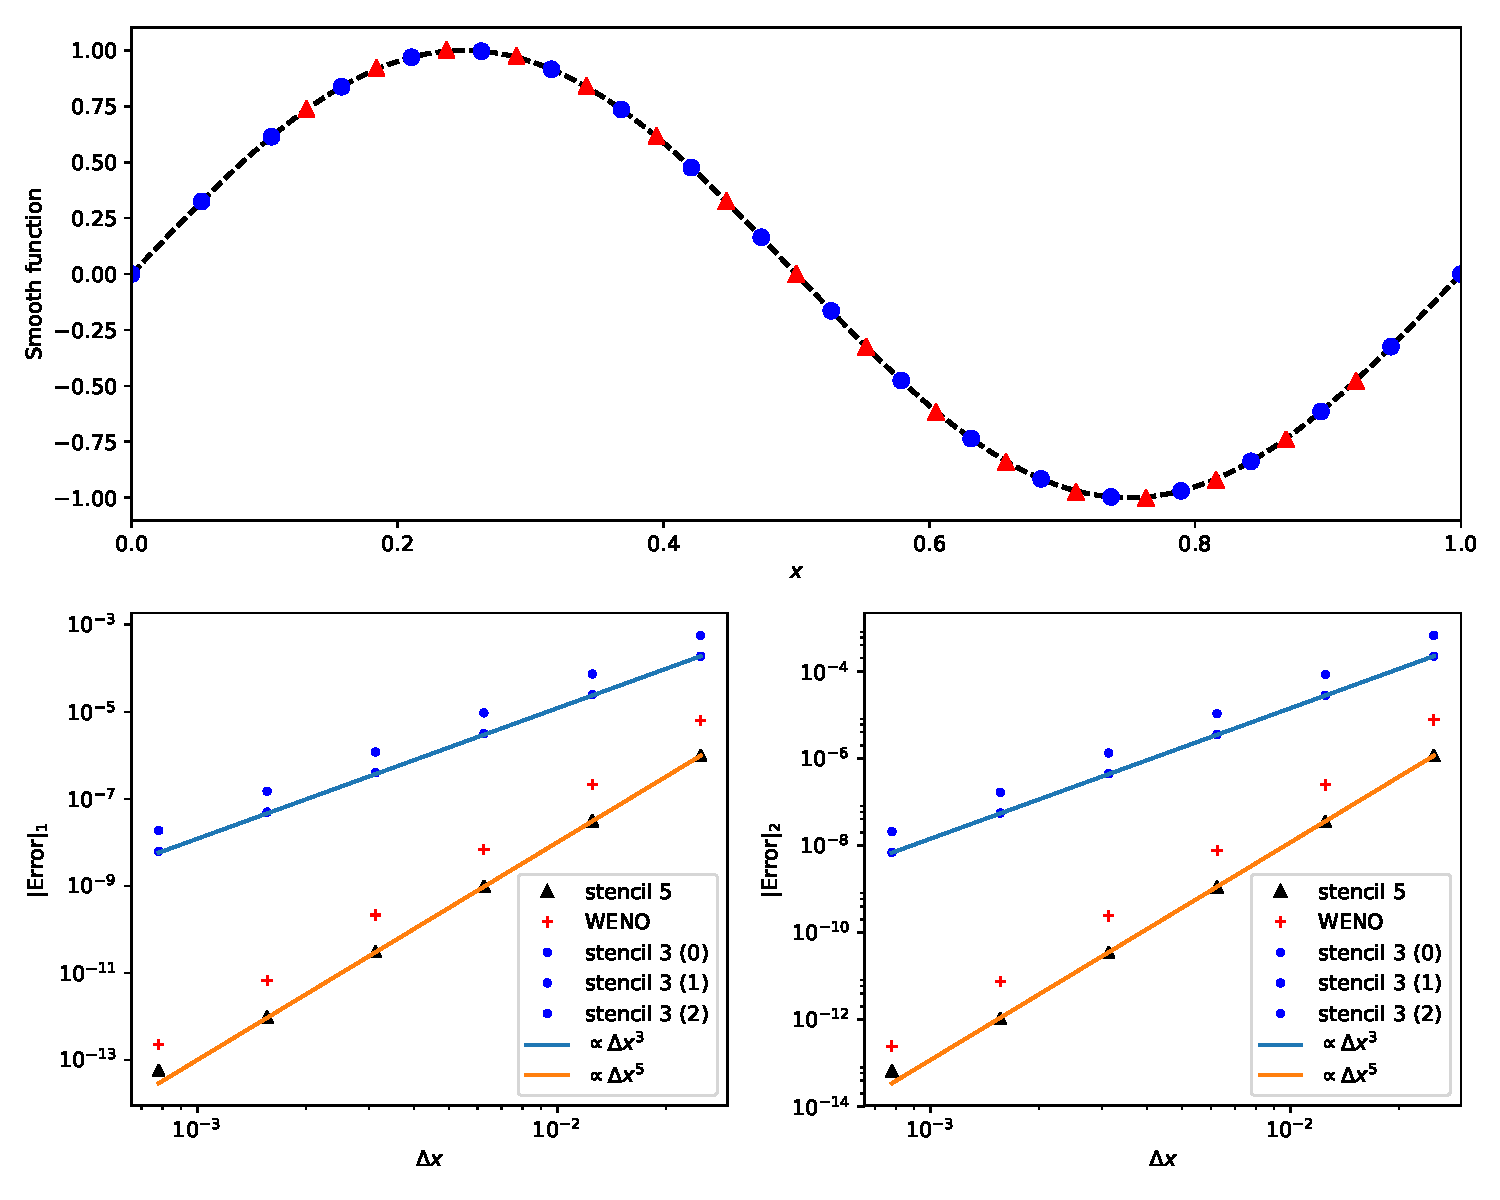
\includegraphics[width=0.96\linewidth]{weno-convergence}
  \caption[Convergence rate of high-order reconstructions]{A smooth sine function is reconstructed on the unit interval from the (integral-average) data, at the blue circles in the top plot, to the right, at the red triangles in the top plot. The convergence rate with grid resolution for the 5 point stencil of equation~\eqref{eq:weno-advection-5pt} and the 3 point stencils of equation~\eqref{eq:weno-advection-3pt} are shown to match expectations in the bottom plots. The error from the WENO reconstruction described in section~\ref{sec:WENO-algorithm} is, on this smooth function, converging with the expected order but larger in magnitude.}
  \label{fig:weno-convergence}
\end{figure}

For the advection equation with constant advection speed $u$, our higher-order
method requires us to find a high-order approximation to $a_{i+\myhalf}$. If we
considered the five points $a_{j}, j \in [i-2, \dots, i+2]$ then we could use
the information from all five of these points to approximate $a_{i+\myhalf}$ as
\begin{equation}
  \label{eq:weno-advection-5pt}
  a^{(\text{Fifth})}_{i+\myhalf} = \tfrac{1}{60} \left( 2 \langle a \rangle_{i-2} - 13 \langle a \rangle_{i-1} + 47 \langle a \rangle_{i} + 27 \langle a \rangle_{i+1} - 3 \langle a \rangle_{i+2} \right) + {\cal O}(\Delta x^5).
\end{equation}
Alternatively we could use only three of the points, in three different ways:
\begin{subequations}
  \label{eq:weno-advection-3pt}
  \begin{align}
    a^{(\text{Third}, 2)}_{i+\myhalf} &= \tfrac{1}{6} \left( 2 \langle a \rangle_{i-2} - 7 \langle a \rangle_{i-1} + 11 \langle a \rangle_{i} \right) + {\cal O}(\Delta x^3), \\
    a^{(\text{Third}, 1)}_{i+\myhalf} &= \tfrac{1}{6} \left( - \langle a \rangle_{i-1} + 5 \langle a \rangle_{i} + 2 \langle a \rangle_{i+1} \right) + {\cal O}(\Delta x^3), \\
    a^{(\text{Third}, 0)}_{i+\myhalf} &= \tfrac{1}{6} \left( 2 \langle a \rangle_{i} + 5 \langle a \rangle_{i+1} - \langle a \rangle_{i+2} \right) + {\cal O}(\Delta x^3).
  \end{align}
\end{subequations}

Which is better? The five point stencil gives higher order accuracy, but
includes information from both sides of the point. This ignores information from
the characteristics and, near discontinuities, will lead to Gibbs oscillations.
The three point stencils give lower accuracy. However, they give us the
flexibility to choose a stencil to avoid discontinuities, possibly using the
characteristic information. The advantages of the higher-order methods are illustrated by reconstructing a smooth function in figure~\ref{fig:weno-convergence}. The disadvantages of using a fixed stencil are illustrated by reconstructing a non-smooth function in figure~\ref{fig:weno-weights}.


\begin{exercise}[ENO stencils]
{Check that equations~\eqref{eq:weno-advection-5pt} and
\eqref{eq:weno-advection-3pt} give the claimed order of accuracy results.}
\end{exercise}

The method of choosing the ``best'' stencil (to avoid discontinuities as far as
possible) is called \emph{Essentially Non-Oscillatory} (ENO) reconstruction. It
is not as accurate as it could be given the size of the stencil it uses, and
the logical branches required to find the ``best'' stencil can reduce
computational performance.

An alternative that avoids the problems of ENO schemes are the \emph{Weighted}
ENO, or WENO, schemes. These use a combination of the possible ENO stencils to
reconstruct $a_{i+\myhalf}$. This relies on the observation that there are
constants $C_k$ such that, for example,
\begin{equation}
  \label{eq:WENO-C-weights}
  a^{(\text{Fifth})}_{i+\myhalf} = \sum_{k=0}^{2} C_k a^{(\text{Third}, r)}_{i+\myhalf}.
\end{equation}

\begin{exercise}[WENO weights]
{Check that the constants $C_0 = \tfrac{3}{10}, C_1 = \tfrac{3}{5}, C_2 =
\tfrac{1}{10}$ make equation~\eqref{eq:WENO-C-weights} consistent with
equations~\eqref{eq:weno-advection-5pt} and \eqref{eq:weno-advection-3pt}.}
\end{exercise}

The WENO methods work by retaining the sum over all stencils as in
equation~\eqref{eq:WENO-C-weights}, but adjusting the weights to avoid
oscillations. Ideally, in regions where the $a^{(0,1)}$ stencils include a
shock but the $a^{(2)}$ stencil does not the weights should be $\tilde{C}_0 = 0
= \tilde{C}_1$ and $\tilde{C}_2 = 1$. In order for this sum to make sense we
will need the weights to add to $1$.

\subsection{WENO algorithm}
\label{sec:WENO-algorithm}

\begin{figure}
  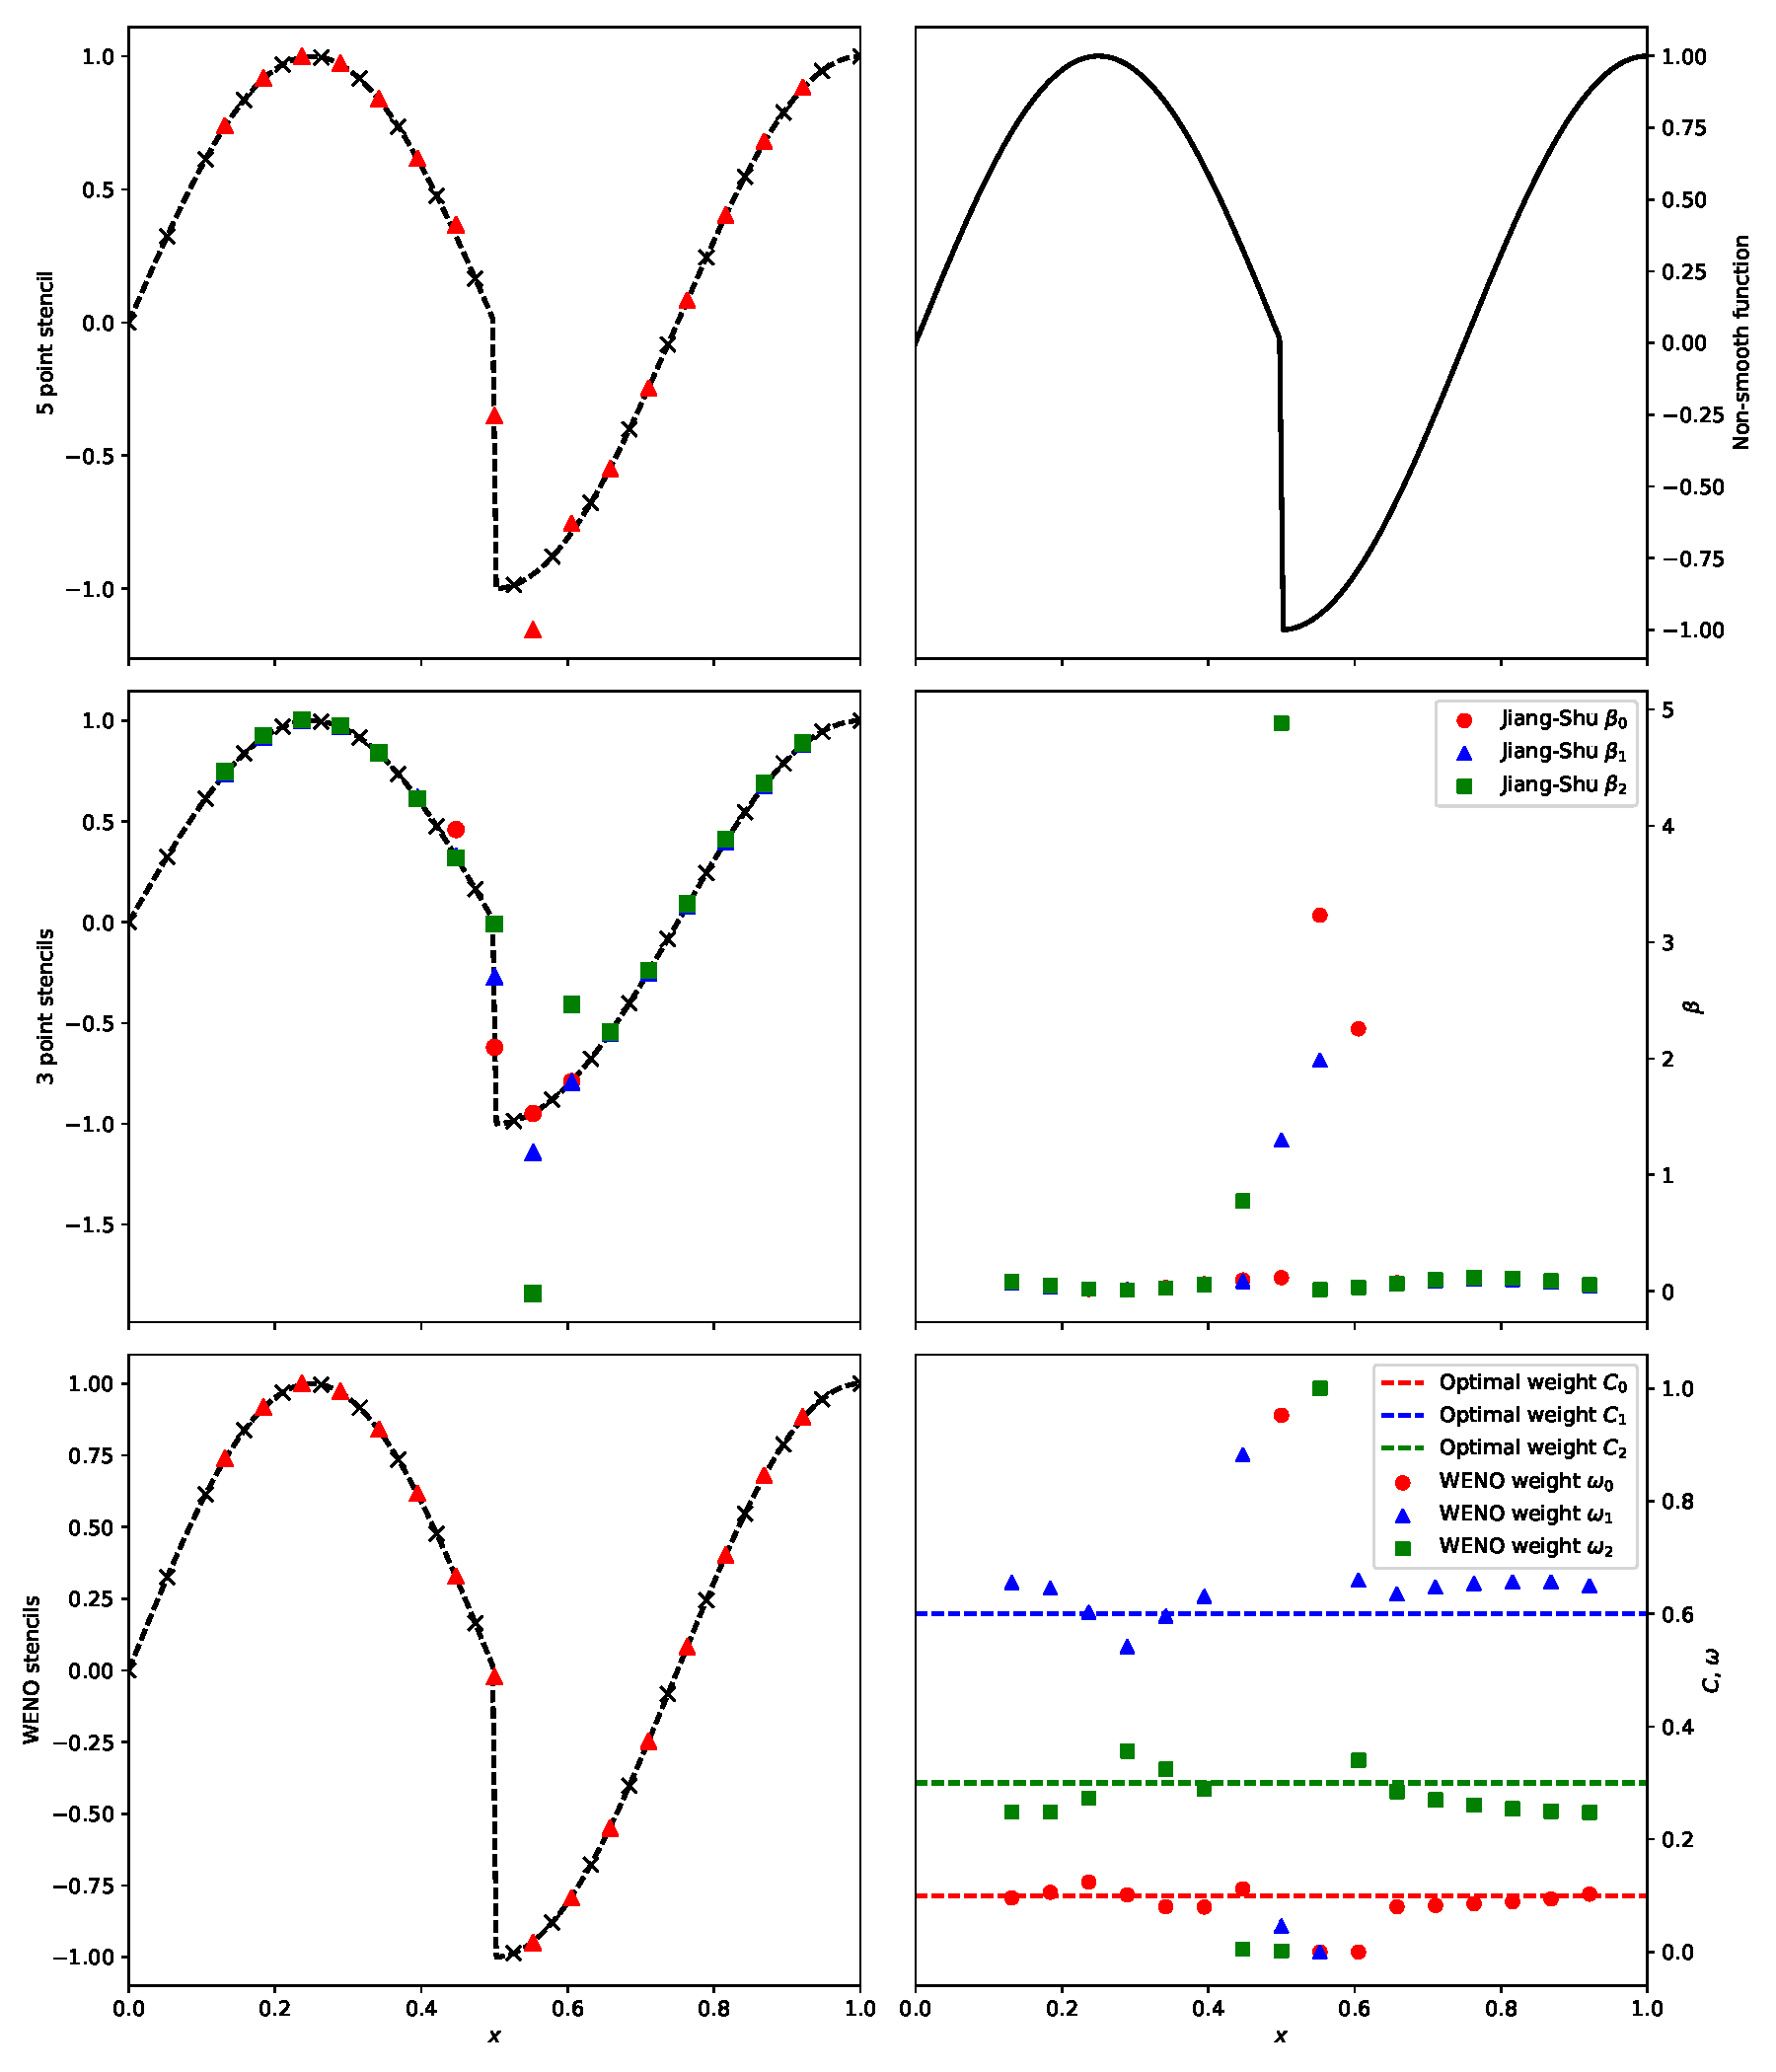
\includegraphics[width=0.96\linewidth]{weno-weights}
  \caption[WENO reconstruction and weights]{A non-smooth function is reconstructed on the unit interval. The 5 point stencil of equation~\eqref{eq:weno-advection-5pt} and the 3 point stencils of equation~\eqref{eq:weno-advection-3pt} both show oscillations near the discontinuity, whilst the WENO reconstruction does not. The WENO algorithm depends on measuring the smoothness of the function. The Jiang-Shu smoothness indicators $\beta$ are mostly zero, but spike near the discontinuity. This feeds into the weight $\omega$ that the WENO algorithm gives to each 3 point stencil it uses. Away from the discontinuity the weights revert to the optimal $C$ weights, but near the discontinuity a single $\omega$ weight dominates meaning only a single 3 point stencil is used.}
  \label{fig:weno-weights}
\end{figure}

We can now write out the full WENO algorithm of order $(2 r - 1)$. The constant
$r$ sets the size of the individual stencils as well as the (optimal) order of
the scheme. This section mostly uses the notation of Gerolymos et al.~\cite{Gerolymos2009}, and we will drop the integral average notation (so $\langle a \rangle_i$ will be denoted $a_i$).

First compute the individual stencils
\begin{equation}
  \label{eq:weno-stencils}
  a_{r, k, i+\myhalf} = \sum_{\ell=0}^{r-1} A_{r, k, \ell} a_{i+k-\ell}, \quad k = 0, \dots, r-1.
\end{equation}
Here the $A_{r, k, \ell}$ terms are constants which, for given scheme accuracy
$r$ are needed to compute the $k^{\text{th}}$ stencil.

We then want to combine these individual stencils to compute the WENO result.
For this we write
\begin{equation}
  \label{eq:weno-reconstruction}
  a_{r, WENO, i+\myhalf} = \sum_{k=0}^{r-1} \omega_{r, k, i+\myhalf} a_{r, k, i+\myhalf}.
\end{equation}
Here the $\omega_{r, k, i+\myhalf}$ terms are the weights that vary from point
to point. They must sum to one, so that we have a convex combination of the
stencils:
\begin{equation}
  \label{eq:weno-convex}
  \sum_{k=1}^{r-1} \omega_{r, k, i+\myhalf} = 1.
\end{equation}
We also want the weights to match the \emph{optimal} weights $C_{r, k}$ in
smooth regions. The optimal weights are defined such that
\begin{equation}
  \label{eq:weno-optimal}
  a_{r, WENO, i+\myhalf} = \sum_{k=0}^{r-1} C_{r, k} a_{r, k, i+\myhalf}
\end{equation}
is accurate to order ${\cal O}(\Delta x^{(2 r - 1)})$ when $q$ is smooth.

The \emph{choice} of how to get from the optimal weights $C_{r, k}$ to the
nonlinear weights $\omega_{r, k, i+\myhalf}$ defines the WENO scheme. The
standard choice of Jiang and Shu is to introduce a measure of the smoothness of
the $k^{\text{th}}$ stencil by computing the sum of the integral averages of
its derivatives from order $1$ up to order $2 r - 1$. For practical
implementation purposes this means computing the \emph{smoothness indicators}
$\beta_{r, k, i+\myhalf}$ as
\begin{equation}
  \label{eq:weno-smoothness}
  \beta_{r, k, i+\myhalf} = \sigma_{r, k, \ell, m} a_{i+k-\ell} a_{i+k-m}.
\end{equation}
The terms $\sigma_{r, k, \ell, m}$ are pre-computed constants which give the
coefficients in the quadratic form for the $k^{\text{th}}$ stencil of width $r$
in the reconstruction. These smoothness indicators are non-negative, and will
be large when the derivatives are large in magnitude. The Jiang and Shu weights
are then set by
\begin{subequations}
  \label{eq:weno-nonlinear-weights}
  \begin{align}
    \label{eq:weno-nonlinear-weights-omega}
    \omega_{r, k, i+\myhalf} &= \frac{\alpha_{r, k, i+\myhalf}}{\sum_{k=0}^{r-1} \alpha_{r, k, i+\myhalf}}, \\
      \label{eq:weno-nonlinear-weights-alpha}
    \alpha_{r, k, i+\myhalf} &= \frac{C_{r, k}}{\epsilon + \beta_{r, k, i+\myhalf}^2}.
  \end{align}
\end{subequations}
Here $\epsilon$ is a small number introduced to avoid division-by-zero problems.
The form of $\omega_{r, k, i+\myhalf}$ in
equation~\eqref{eq:weno-nonlinear-weights-omega} guarantees that the convex sum
condition in equation~\eqref{eq:weno-convex} holds. The form of $\alpha_{r, k,
i+\myhalf}$ ensures that when all the smoothness indicators $\beta_{r, k,
i+\myhalf}$ are the same magnitude the weights $\omega_{r, k, i+\myhalf}$ will
match the optimal weights $C_{r, k}$, but when a smoothness indicator is large
(i.e., when the associated stencil has large derivatives, typically associated
with discontinuities), the contribution of its associated stencil will be small.
An example of this is shown in figure~\ref{fig:weno-weights}.

Finally, we note that this method has reconstructed $a_{i+\myhalf}$ from the
left. For the advection equation case where the advection speed $u$ is positive
this is all we need: the characteristic information tells us that we should use
this reconstruction. In the case where the advection speed is negative we
should reconstruct from the right. In the implementation it is easiest to
implement only one reconstruction direction and pass the data in in reverse
order.


\begin{exercise}[WENO reconstruction]
{Taking the values for the $C$, $A$ and $\sigma$ constants from Gerolymos et
al.\ or Shu's review~\cite{Shu1997}, construct a WENO reconstruction method for
$r=2$. Check your results on smooth and non-smooth functions.}
\end{exercise}

\subsection{Implementation issues with WENO schemes}
\label{sec:weno-implementation}

A convergence test on the WENO schemes with $r=3$ and $r=5$ is shown in
figure~\ref{fig:weno-converge-gaussian-rk4}. This should be compared to
figure~\ref{fig:advnorm}, as in both a Gaussian profile is advected five
times around a periodic domain. The WENO schemes show higher absolute accuracy
for moderate size grids ($N \gtrsim 100$) and show faster convergence.

However, it is clear that whilst the $r=3$ method converges at fifth order as
expected, the $r=5$ WENO method does not converge at ninth order but at fourth
order. This is explained by the time integrator. We remember that any solver
has an error both from the spatial and the time discretization. In
figure~\ref{fig:weno-converge-gaussian-rk4} the time integrator is the classic
fourth order Runge-Kutta, and it is the error from this integrator that is
dominating.

To confirm this, figure~\ref{fig:weno-converge-gaussian} uses the eigth order
Dormand-Price Runge-Kutta method with adaptive step size control (using the
\texttt{scipy.integrate.ode} routine). Here we see high order convergence for
all $r$, and in each case the convergence rate is $2 r - 2$ for \textbf{no
reason I can understand}.

\begin{figure}[t]
\centering
% figure generated by hydro_examples/advection/weno.py
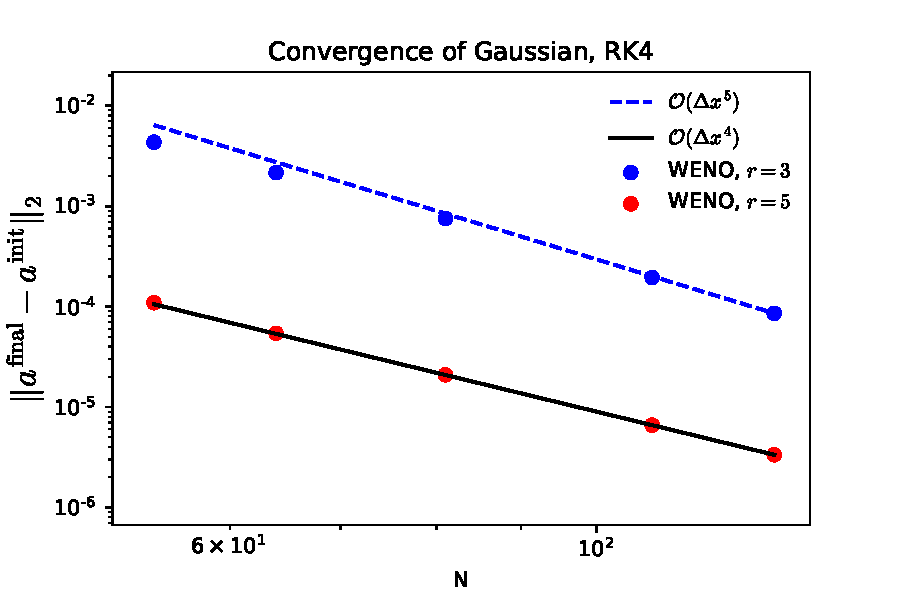
\includegraphics[width=0.8\linewidth]{weno-converge-gaussian-rk4}
\caption[High order WENO convergence rates for linear advection]
{\label{fig:weno-converge-gaussian-rk4} WENO solutions for advecting a Gaussian five periods, using two different orders. A fourth order Runge-Kutta method is used for time evolution. For $r=3$ we see the expected fifth ($2 r - 1$) order convergence. For $r=5$ we see fourth order, rather than the expected ninth order, convergence. This is as the error from the time integrator dominates. \\
\hydroexdoit{\href{https://github.com/zingale/hydro_examples/blob/master/advection/weno.py}{weno.py}}}
\end{figure}
%

\begin{figure}[t]
\centering
% figure generated by hydro_examples/advection/weno.py
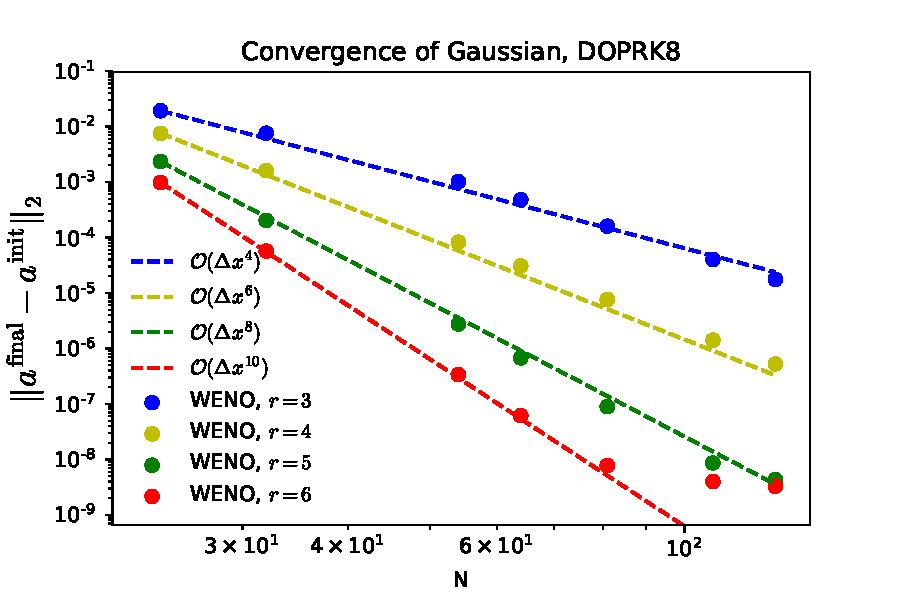
\includegraphics[width=0.8\linewidth]{weno-converge-gaussian}
\caption[Very high order WENO convergence rates for linear advection]
{\label{fig:weno-converge-gaussian} WENO solutions for advecting a Gaussian one periods, using four different orders. An eighth order Dormand-Price Runge-Kutta method is used for time evolution. This minimizes the time integrator error and we see convergence at order $2 r - 2$ for all schemes, although the time integrator error eventually shows in the highest order case. \\
\hydroexdoit{\href{https://github.com/zingale/hydro_examples/blob/master/advection/weno.py}{weno.py}}}
\end{figure}
%
